% Digital Logic Report Template
% Created: 2020-01-10, John Miller

%==========================================================
%=========== Document Setup  ==============================

% Formatting defined by class file
\documentclass[11pt]{article}

% ---- Document formatting ----
\usepackage[margin=1in]{geometry}	% Narrower margins
\usepackage{booktabs}				% Nice formatting of tables
\usepackage{graphicx}				% Ability to include graphics

%\setlength\parindent{0pt}	% Do not indent first line of paragraphs 
\usepackage[parfill]{parskip}		% Line space b/w paragraphs
%	parfill option prevents last line of pgrph from being fully justified

% Parskip package adds too much space around titles, fix with this
\RequirePackage{titlesec}
\titlespacing\section{0pt}{8pt plus 4pt minus 2pt}{3pt plus 2pt minus 2pt}
\titlespacing\subsection{0pt}{4pt plus 4pt minus 2pt}{-2pt plus 2pt minus 2pt}
\titlespacing\subsubsection{0pt}{2pt plus 4pt minus 2pt}{-6pt plus 2pt minus 2pt}

% ---- Hyperlinks ----
\usepackage[colorlinks=true,urlcolor=blue]{hyperref}	% For URL's. Automatically links internal references.

% ---- Code listings ----
\usepackage{listings} 					% Nice code layout and inclusion
\usepackage[usenames,dvipsnames]{xcolor}	% Colors (needs to be defined before using colors)

% Define custom colors for listings
\definecolor{listinggray}{gray}{0.98}		% Listings background color
\definecolor{rulegray}{gray}{0.7}			% Listings rule/frame color

% Style for Verilog
\lstdefinestyle{Verilog}{
	language=Verilog,					% Verilog
	backgroundcolor=\color{listinggray},	% light gray background
	rulecolor=\color{blue}, 			% blue frame lines
	frame=tb,							% lines above & below
	linewidth=\columnwidth, 			% set line width
	basicstyle=\small\ttfamily,	% basic font style that is used for the code	
	breaklines=true, 					% allow breaking across columns/pages
	tabsize=3,							% set tab size
	commentstyle=\color{gray},	% comments in italic 
	stringstyle=\upshape,				% strings are printed in normal font
	showspaces=false,					% don't underscore spaces
}

% How to use: \Verilog[listing_options]{file}
\newcommand{\Verilog}[2][]{%
	\lstinputlisting[style=Verilog,#1]{#2}
}




%======================================================
%=========== Body  ====================================
\begin{document}

\title{ELC 2137 Lab 09: ALU with Input Register}
\author{Abigail Joseph}

\maketitle


\section*{Summary}

In this lab, we constructed two modules, a register and an ALU. The register uses a clock input to store data. The ALU implements various logical and arithmetic operations using one input to determine which operation and two others upon which the operation is done. One ALU and two registers were combined in a top-level module to connect their inputs to switches on the Basys3 and their outputs to LEDs to display the various operations as binary numbers in the LEDs.  


\section*{Code}

\Verilog[firstline=23, caption=Register ,label=code:file_1]{register.sv}
\Verilog[firstline=23, caption=Register Testbench ,label=code:file_2]{register_test.sv}
\Verilog[firstline=23, caption=ALU ,label=code:file_3]{alu.sv}
\Verilog[firstline=23, caption=ALU Testbench ,label=code:file_4]{alu_test.sv}
\Verilog[firstline=23, caption=Top-Level File ,label=code:file_5]{top_lab9.sv}

\section*{Results}


	
\begin{table*}[ht]\centering
	\caption{\textit register expected results table}
	\label{ALU:tbl:register_ERT}\medskip
	\begin{tabular}{l|rrrrrrrrrrr}
		Time (ns): & 0-5 & 5-10 & 10-15 & 15-20 & 20-25 & 25-30 & 30-35 & 35-40 & 40-45 & 45-50 & 50-55 \\
		\midrule
		D (hex) & 0 & 0 	  & A & A & 3 	    & 3 	  & 0 	    & 0 & 0$\to$6 & 6 & 6 \\
		clk     & 0 & 1 	  & 0 & 1 & 0 	    & 1 	  & 0 	    & 1 & 0 	  & 1 & 0 \\
		en  	& 0 & 0 	  & 1 & 1 & 1$\to$0 & 0$\to$1 & 1$\to$0 & 0 & 0$\to$1 & 1 & 1 \\
		rst 	& 0 & 0$\to$1 & 0 & 0 & 0 		& 0 	  & 0		& 0 & 0		  & 0 & 0 \\
		\midrule
		Q (hex) & X & X$\to$0 & 0 & A & A & A & A & A & 6 & 6 & \\
		\bottomrule
	\end{tabular}
\end{table*}

\begin{figure}[ht] \centering	
	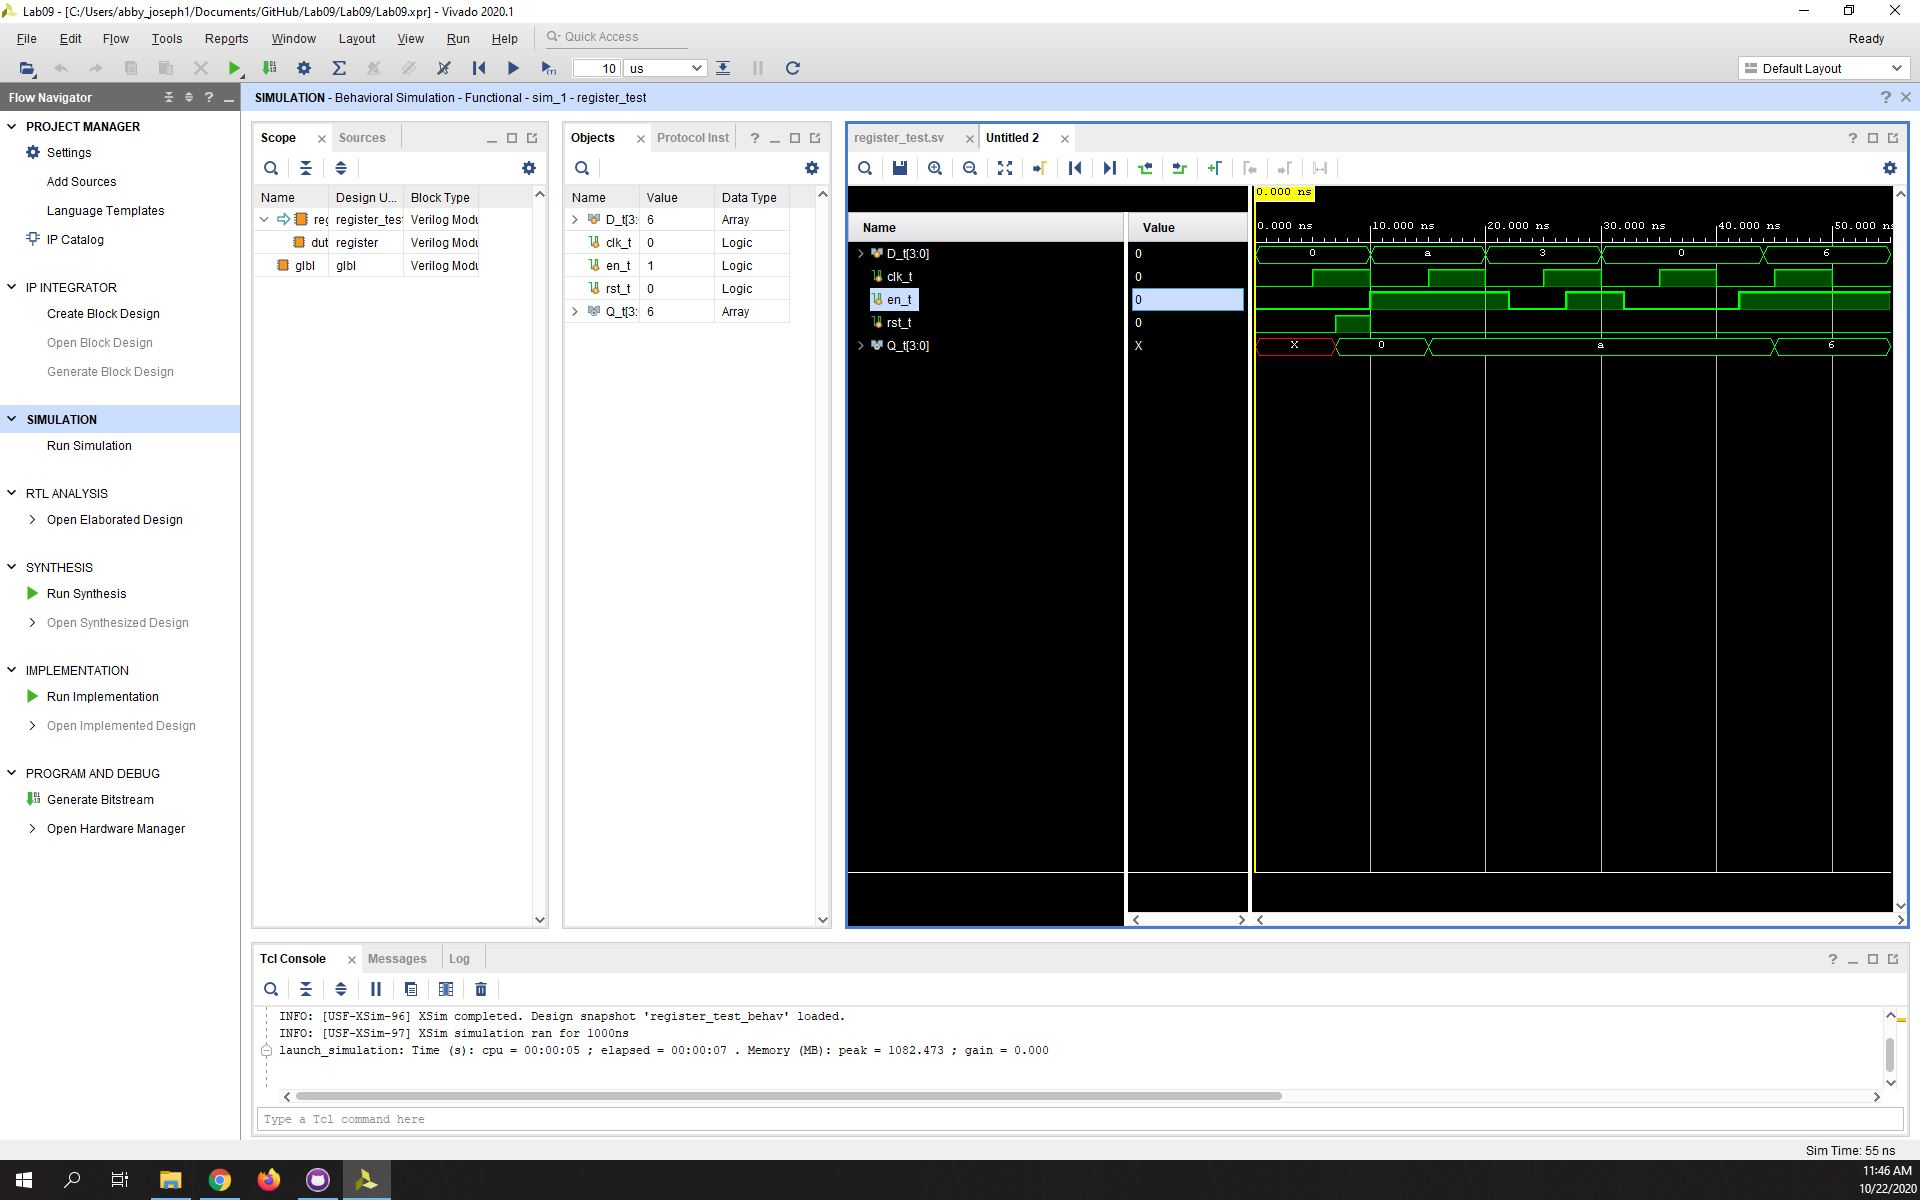
\includegraphics[width=1\textwidth,trim=21cm 19cm 0cm 6cm,clip]{register_test_scrn}
	\caption{Register Simulation}
	\label{fig:img1}
\end{figure}

\begin{table*}[ht]\centering
	\caption{\textit alu expected results table skeleton}
	\label{ALU:tbl:alu_ERT}\medskip
	\begin{tabular}{l|rrrrrr}
		Time (ns): & 0-10 & 10-20 & 20-30 & 30-40 & 40-50 & 50-60 \\
		\midrule
		in0 & 1001 0100 & 1111 1111 & 0011 1010 & 1100 0011 & 1010 0101 & 0000 0001 \\
		in1 & 0011 0000 & 0000 0001 & 0101 1100 & 1011 0100 & 1100 1110 & 0000 0000 \\
		op	& 0000 & 0001 & 0010 & 0011 & 0100 & 1000 \\
		\midrule
		out & 1100 0100 & 1111 1110 & 0001 1000 & 1111 0111 & 0110 1011 & 0000 0001 \\
		\bottomrule
	\end{tabular}
\end{table*}

\begin{figure}[ht] \centering	
	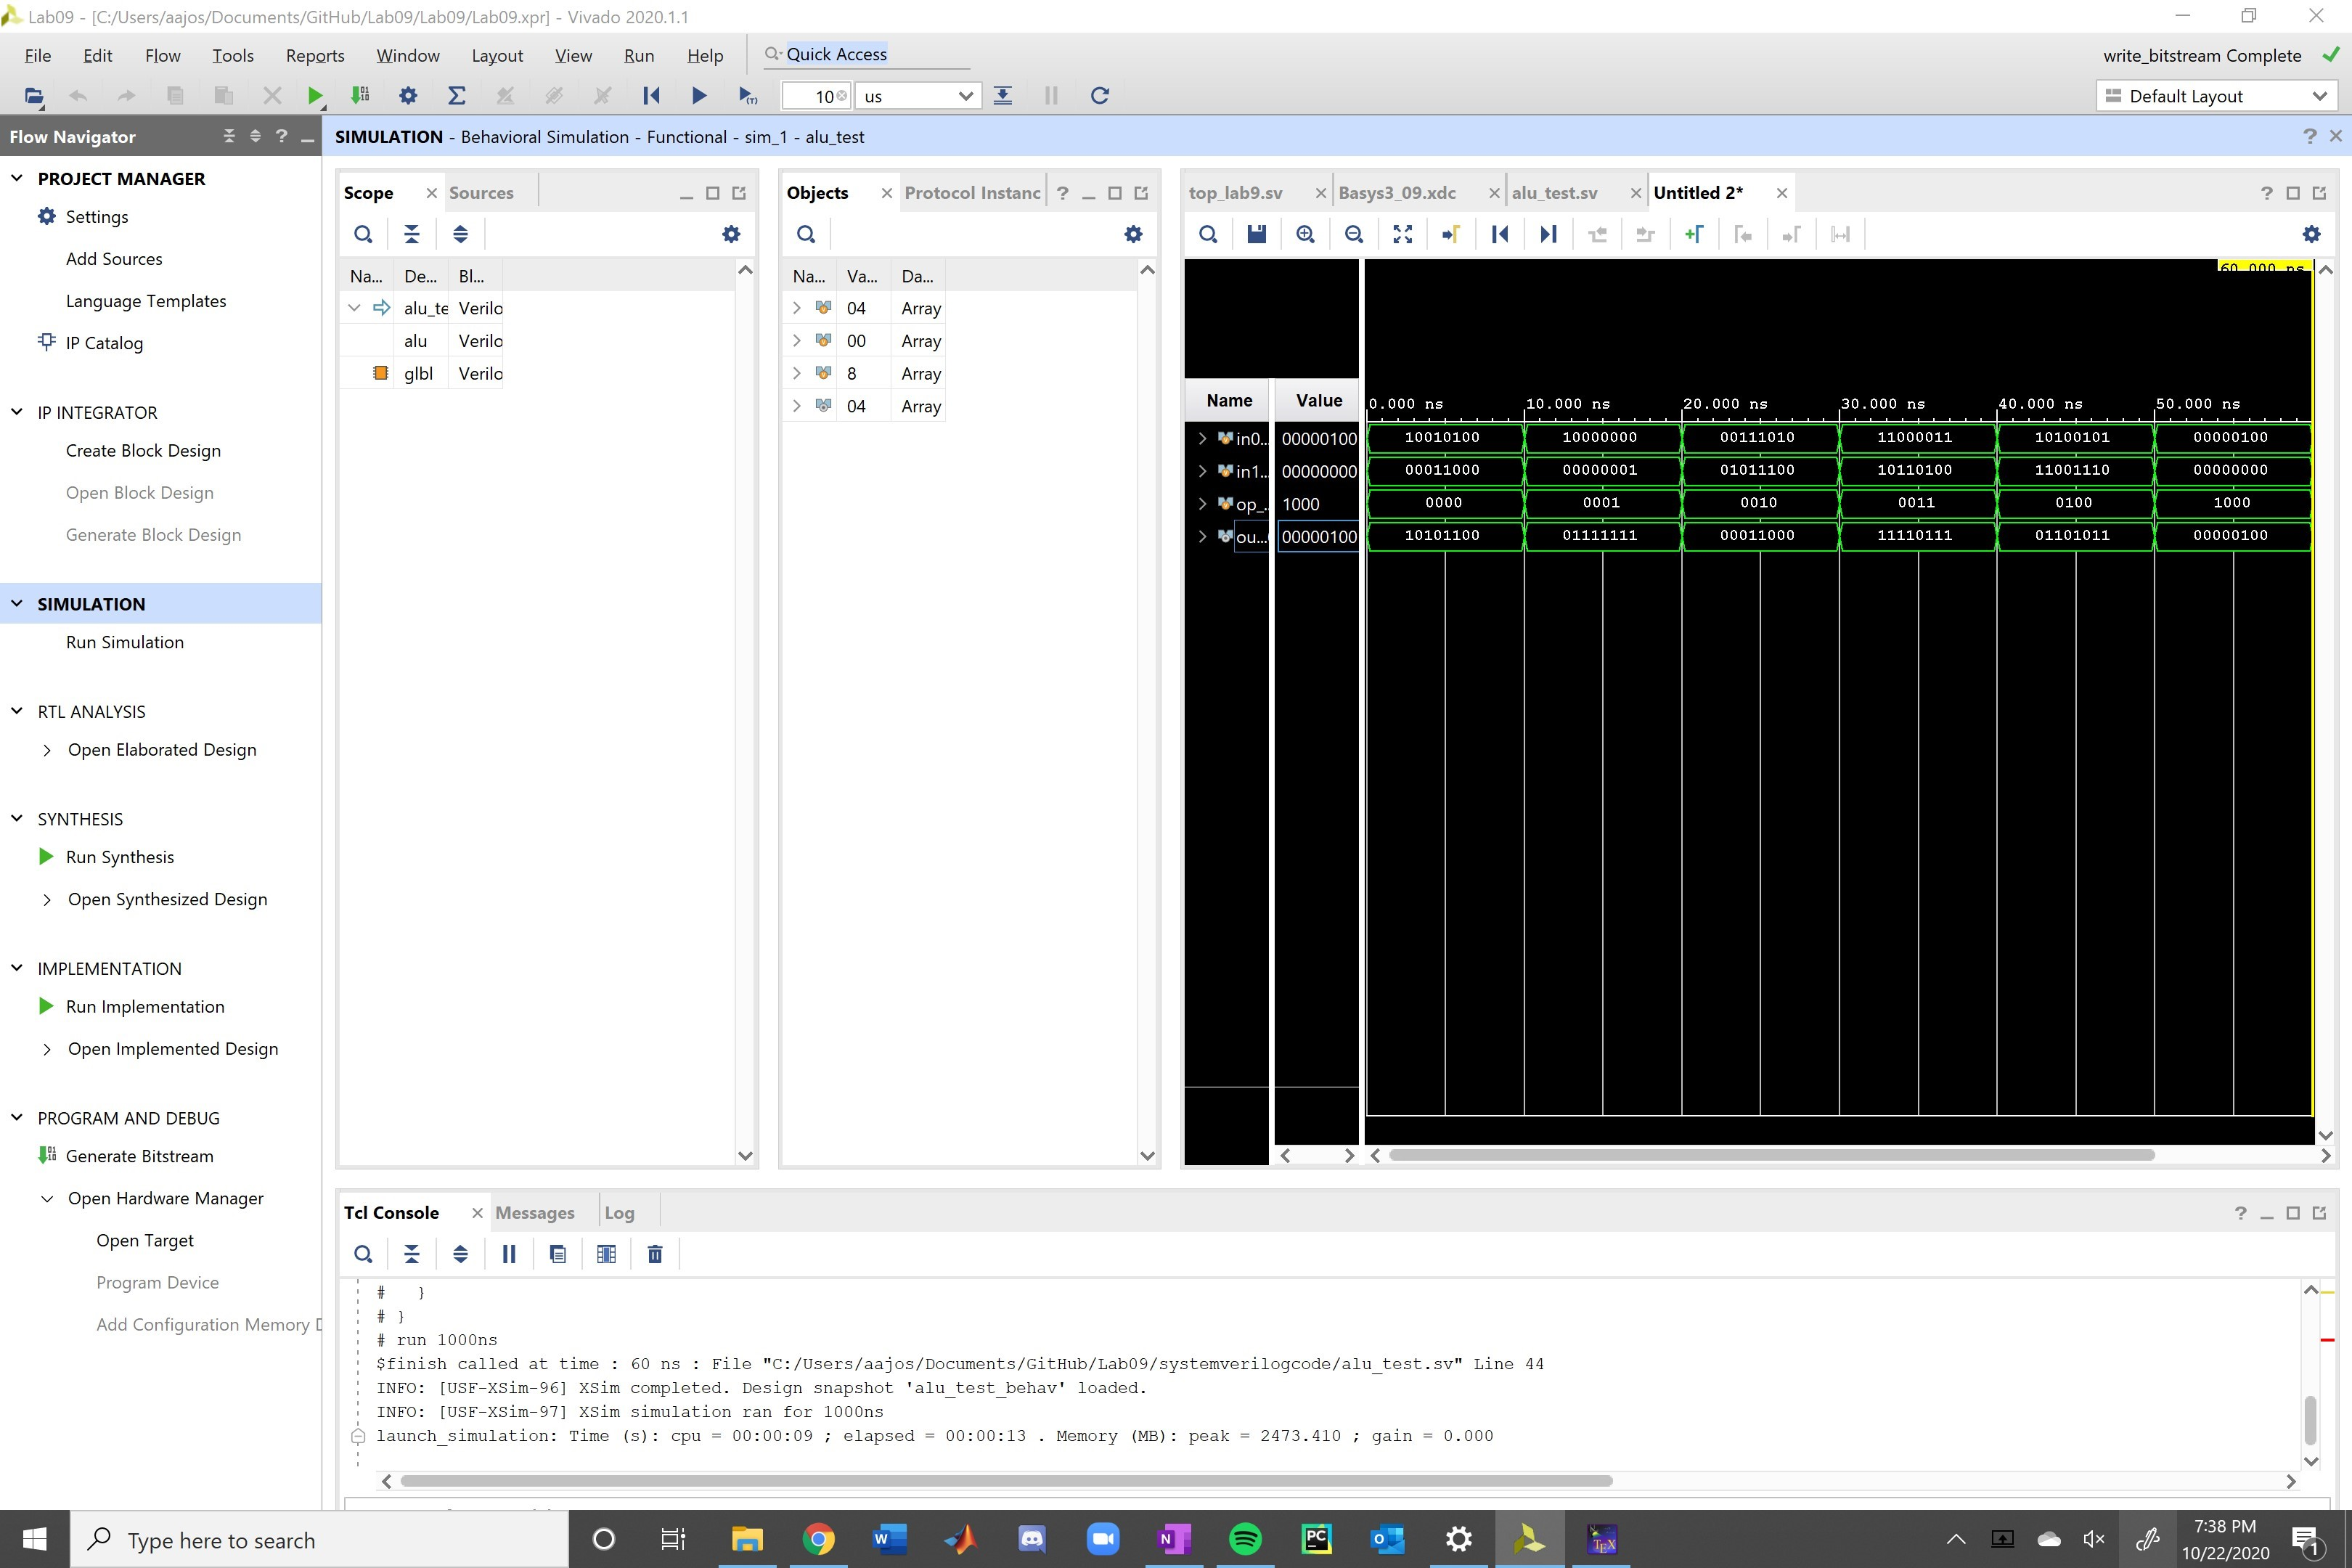
\includegraphics[width=1\textwidth,trim=19cm 15cm 0cm 6cm,clip]{alu_test_scrn}
	\caption{ALU Simulation}
	\label{fig:img2}
\end{figure}

\begin{figure}[ht]\centering
	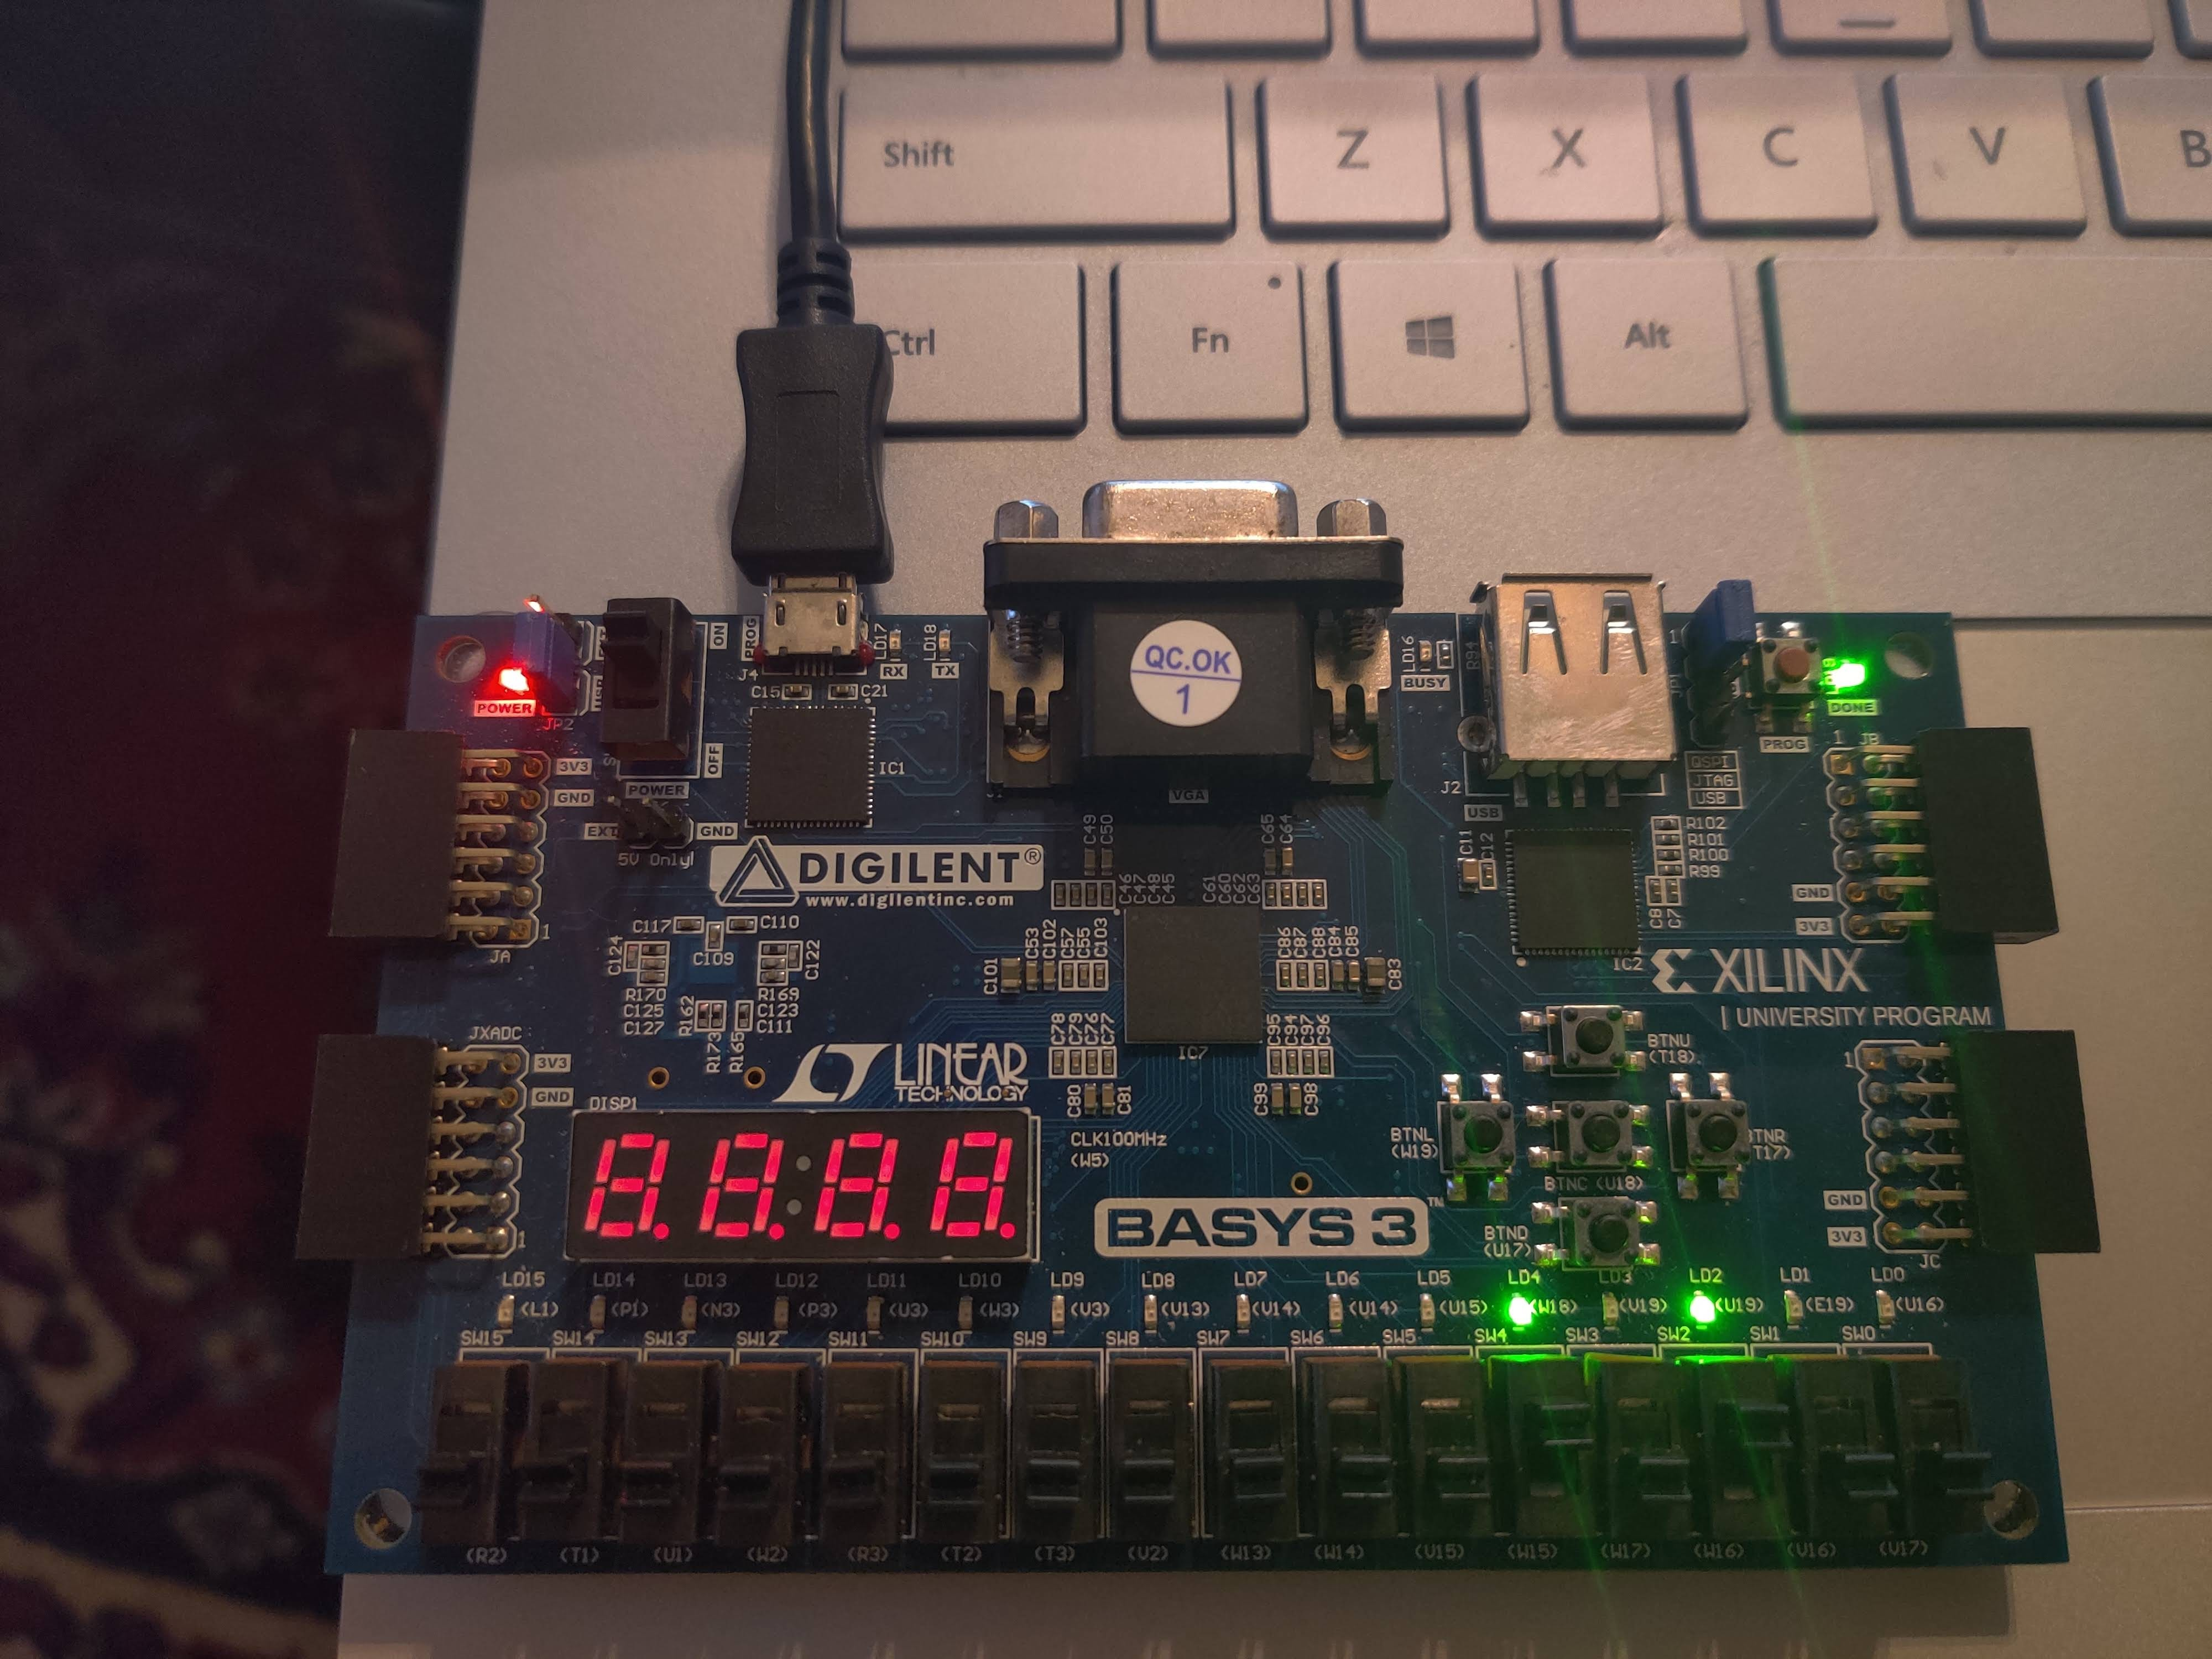
\includegraphics[width=.5\textwidth]{board1}
	\caption{10100}
	\label{fig:b3_1}			
\end{figure}

\begin{figure}[ht]\centering
	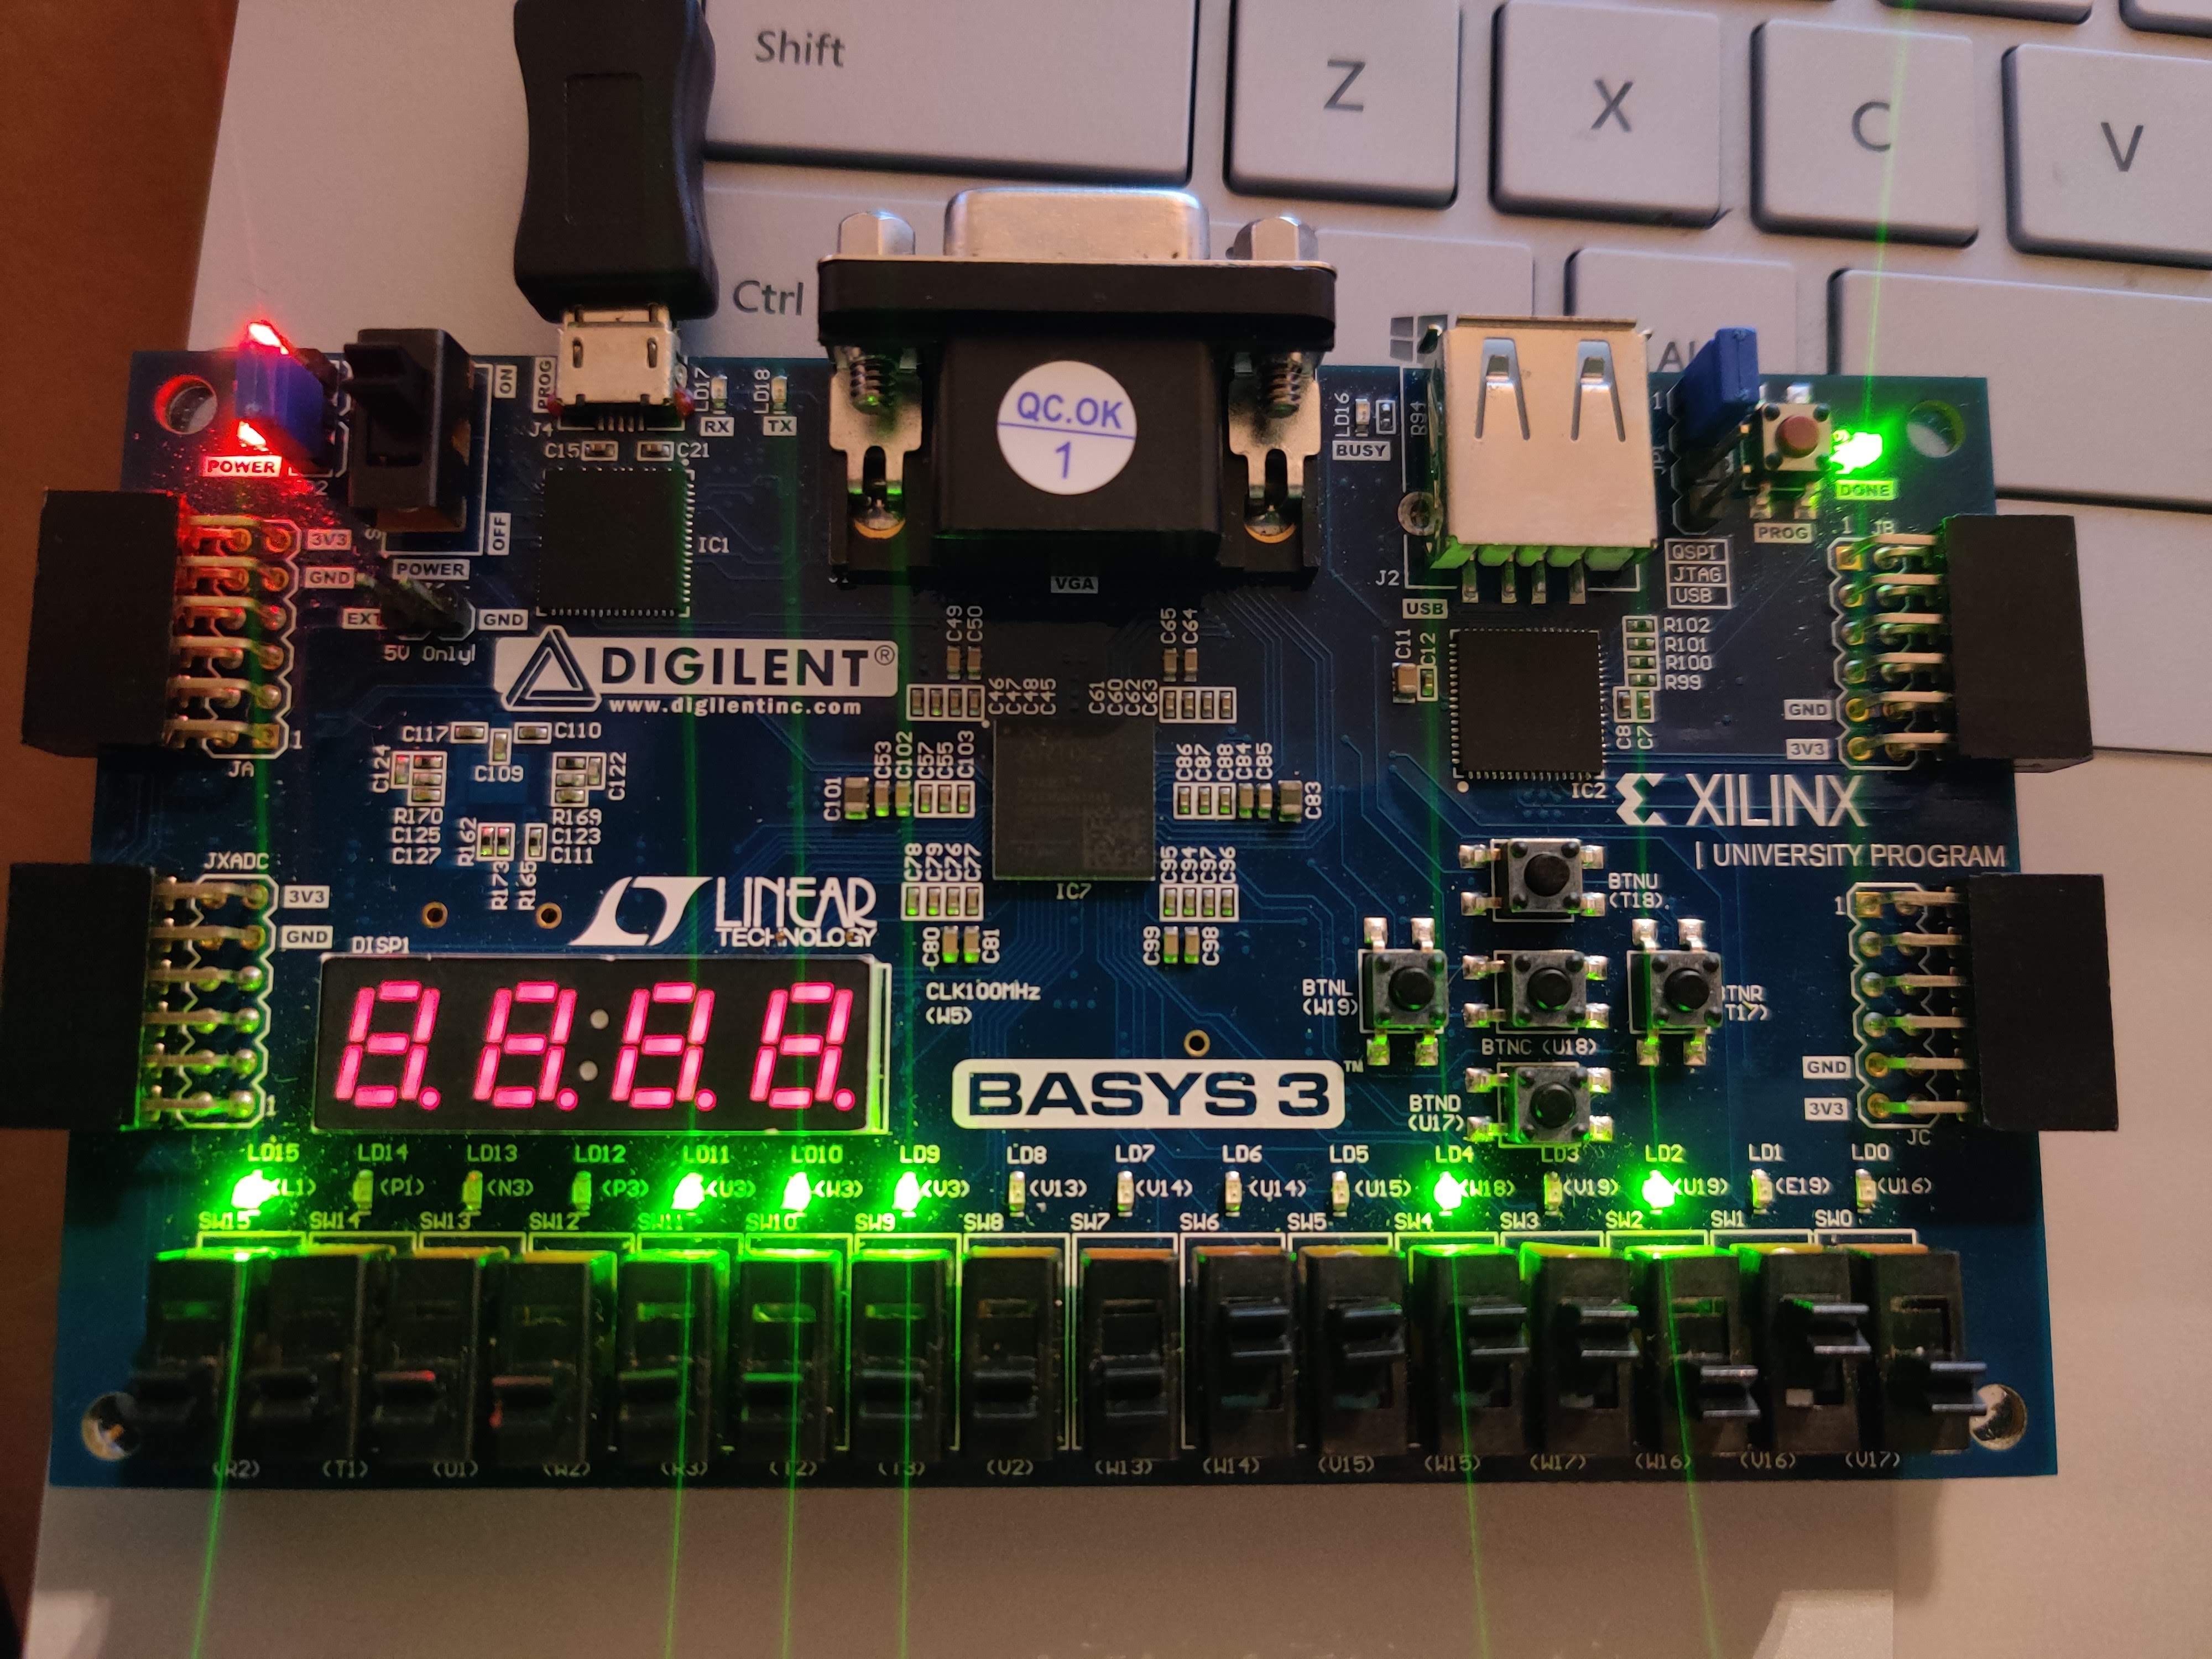
\includegraphics[width=.5\textwidth]{board2}
	\caption{10100+1111010}
	\label{fig:b3_2}			
\end{figure}

\begin{figure}[ht]\centering
	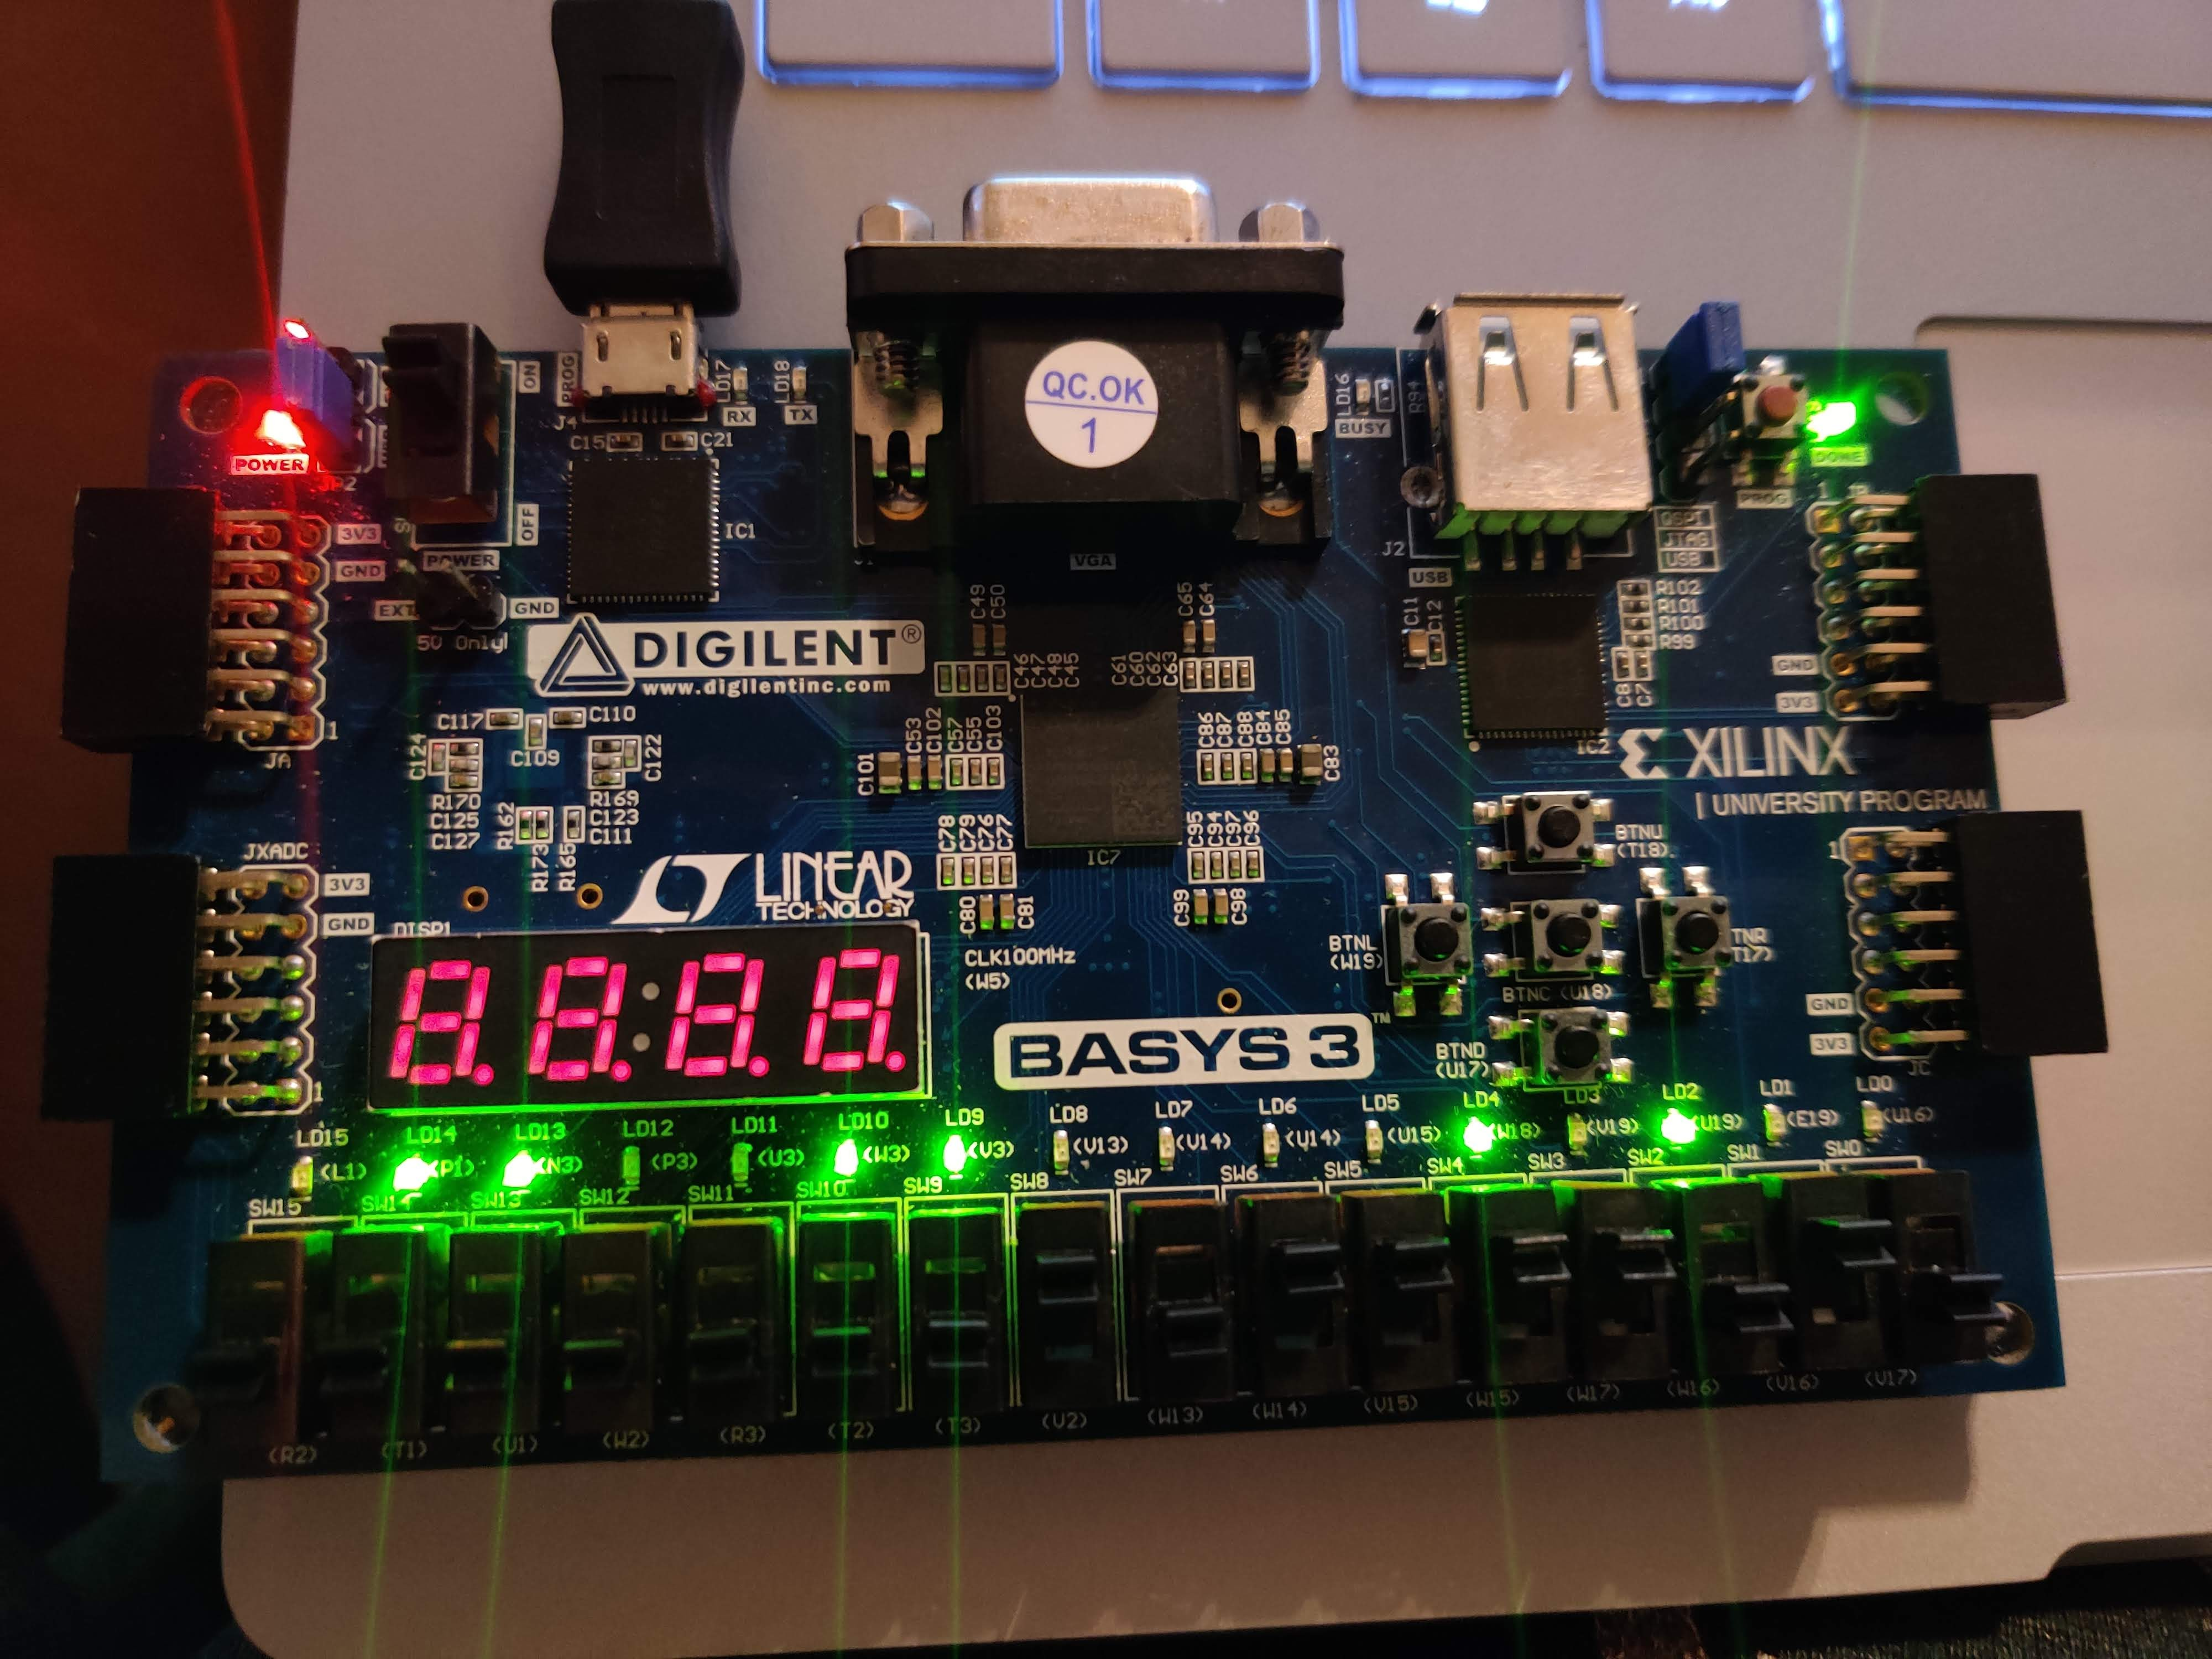
\includegraphics[width=.5\textwidth]{board3}
	\caption{10100-1111010}
	\label{fig:b3_3}			
\end{figure}

\begin{figure}[ht]\centering
	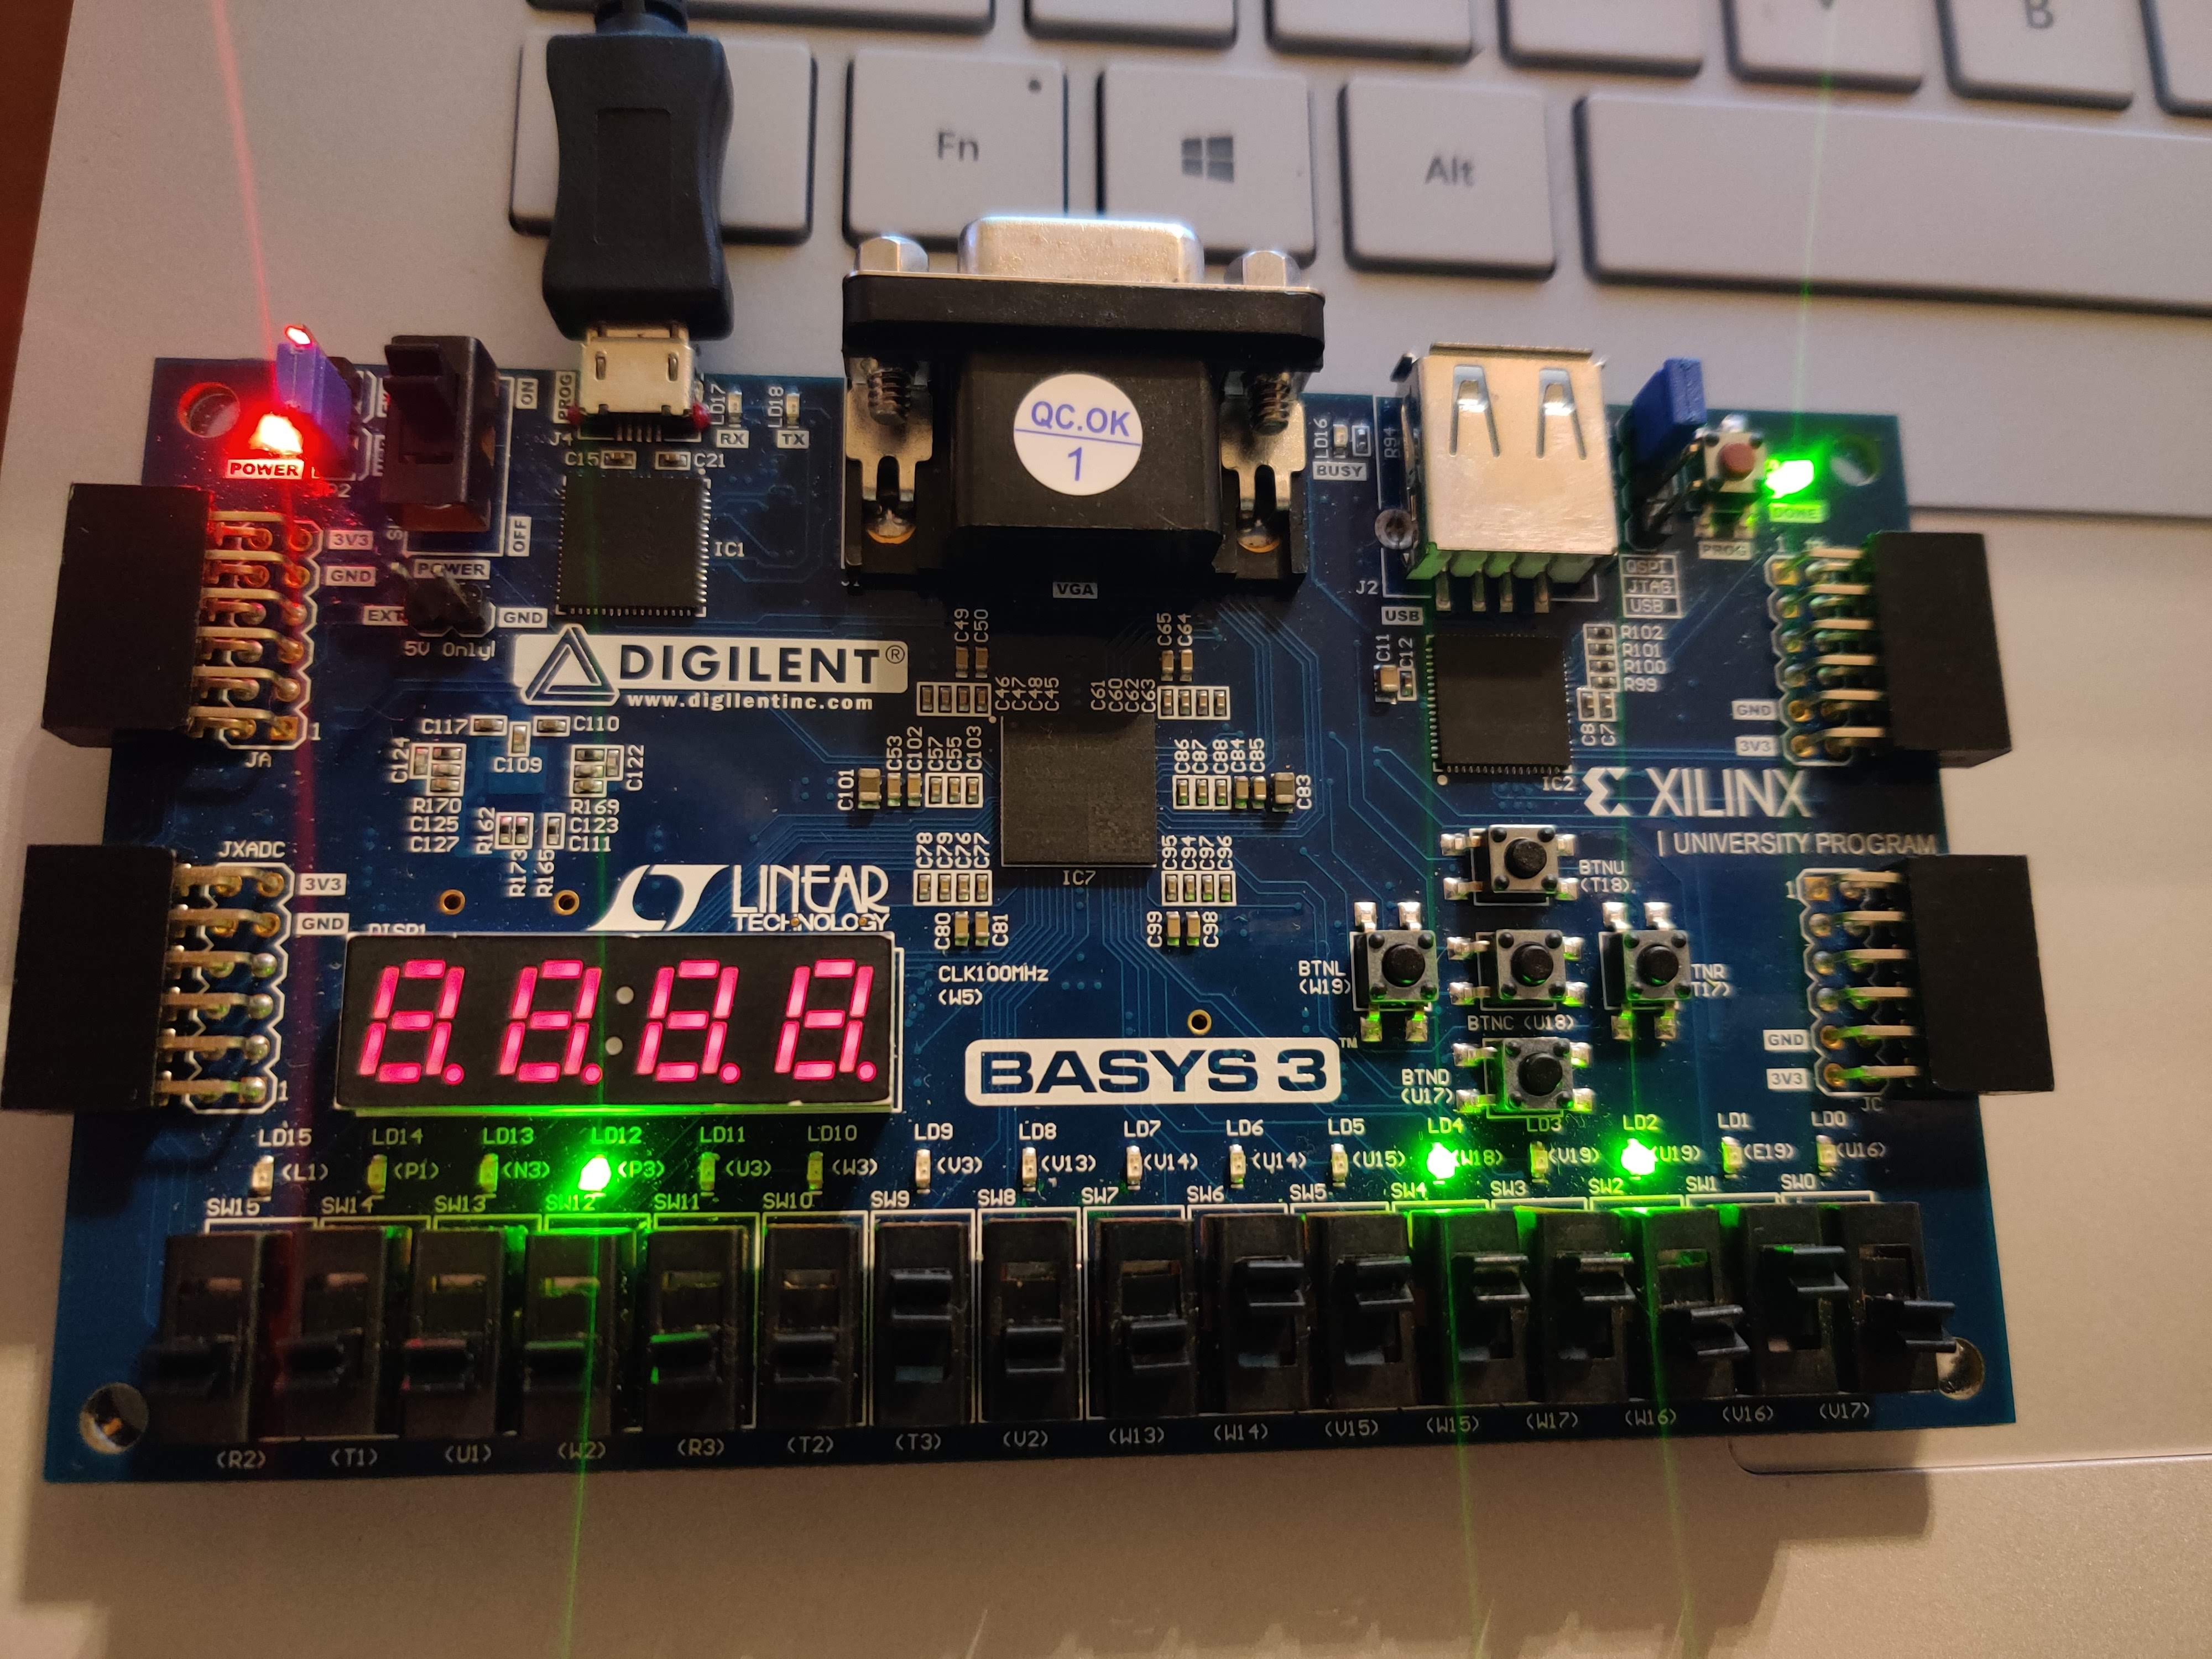
\includegraphics[width=.5\textwidth]{board4}
	\caption{10100 AND 1111010}
	\label{fig:b3_4}			
\end{figure}

\begin{figure}[ht]\centering
	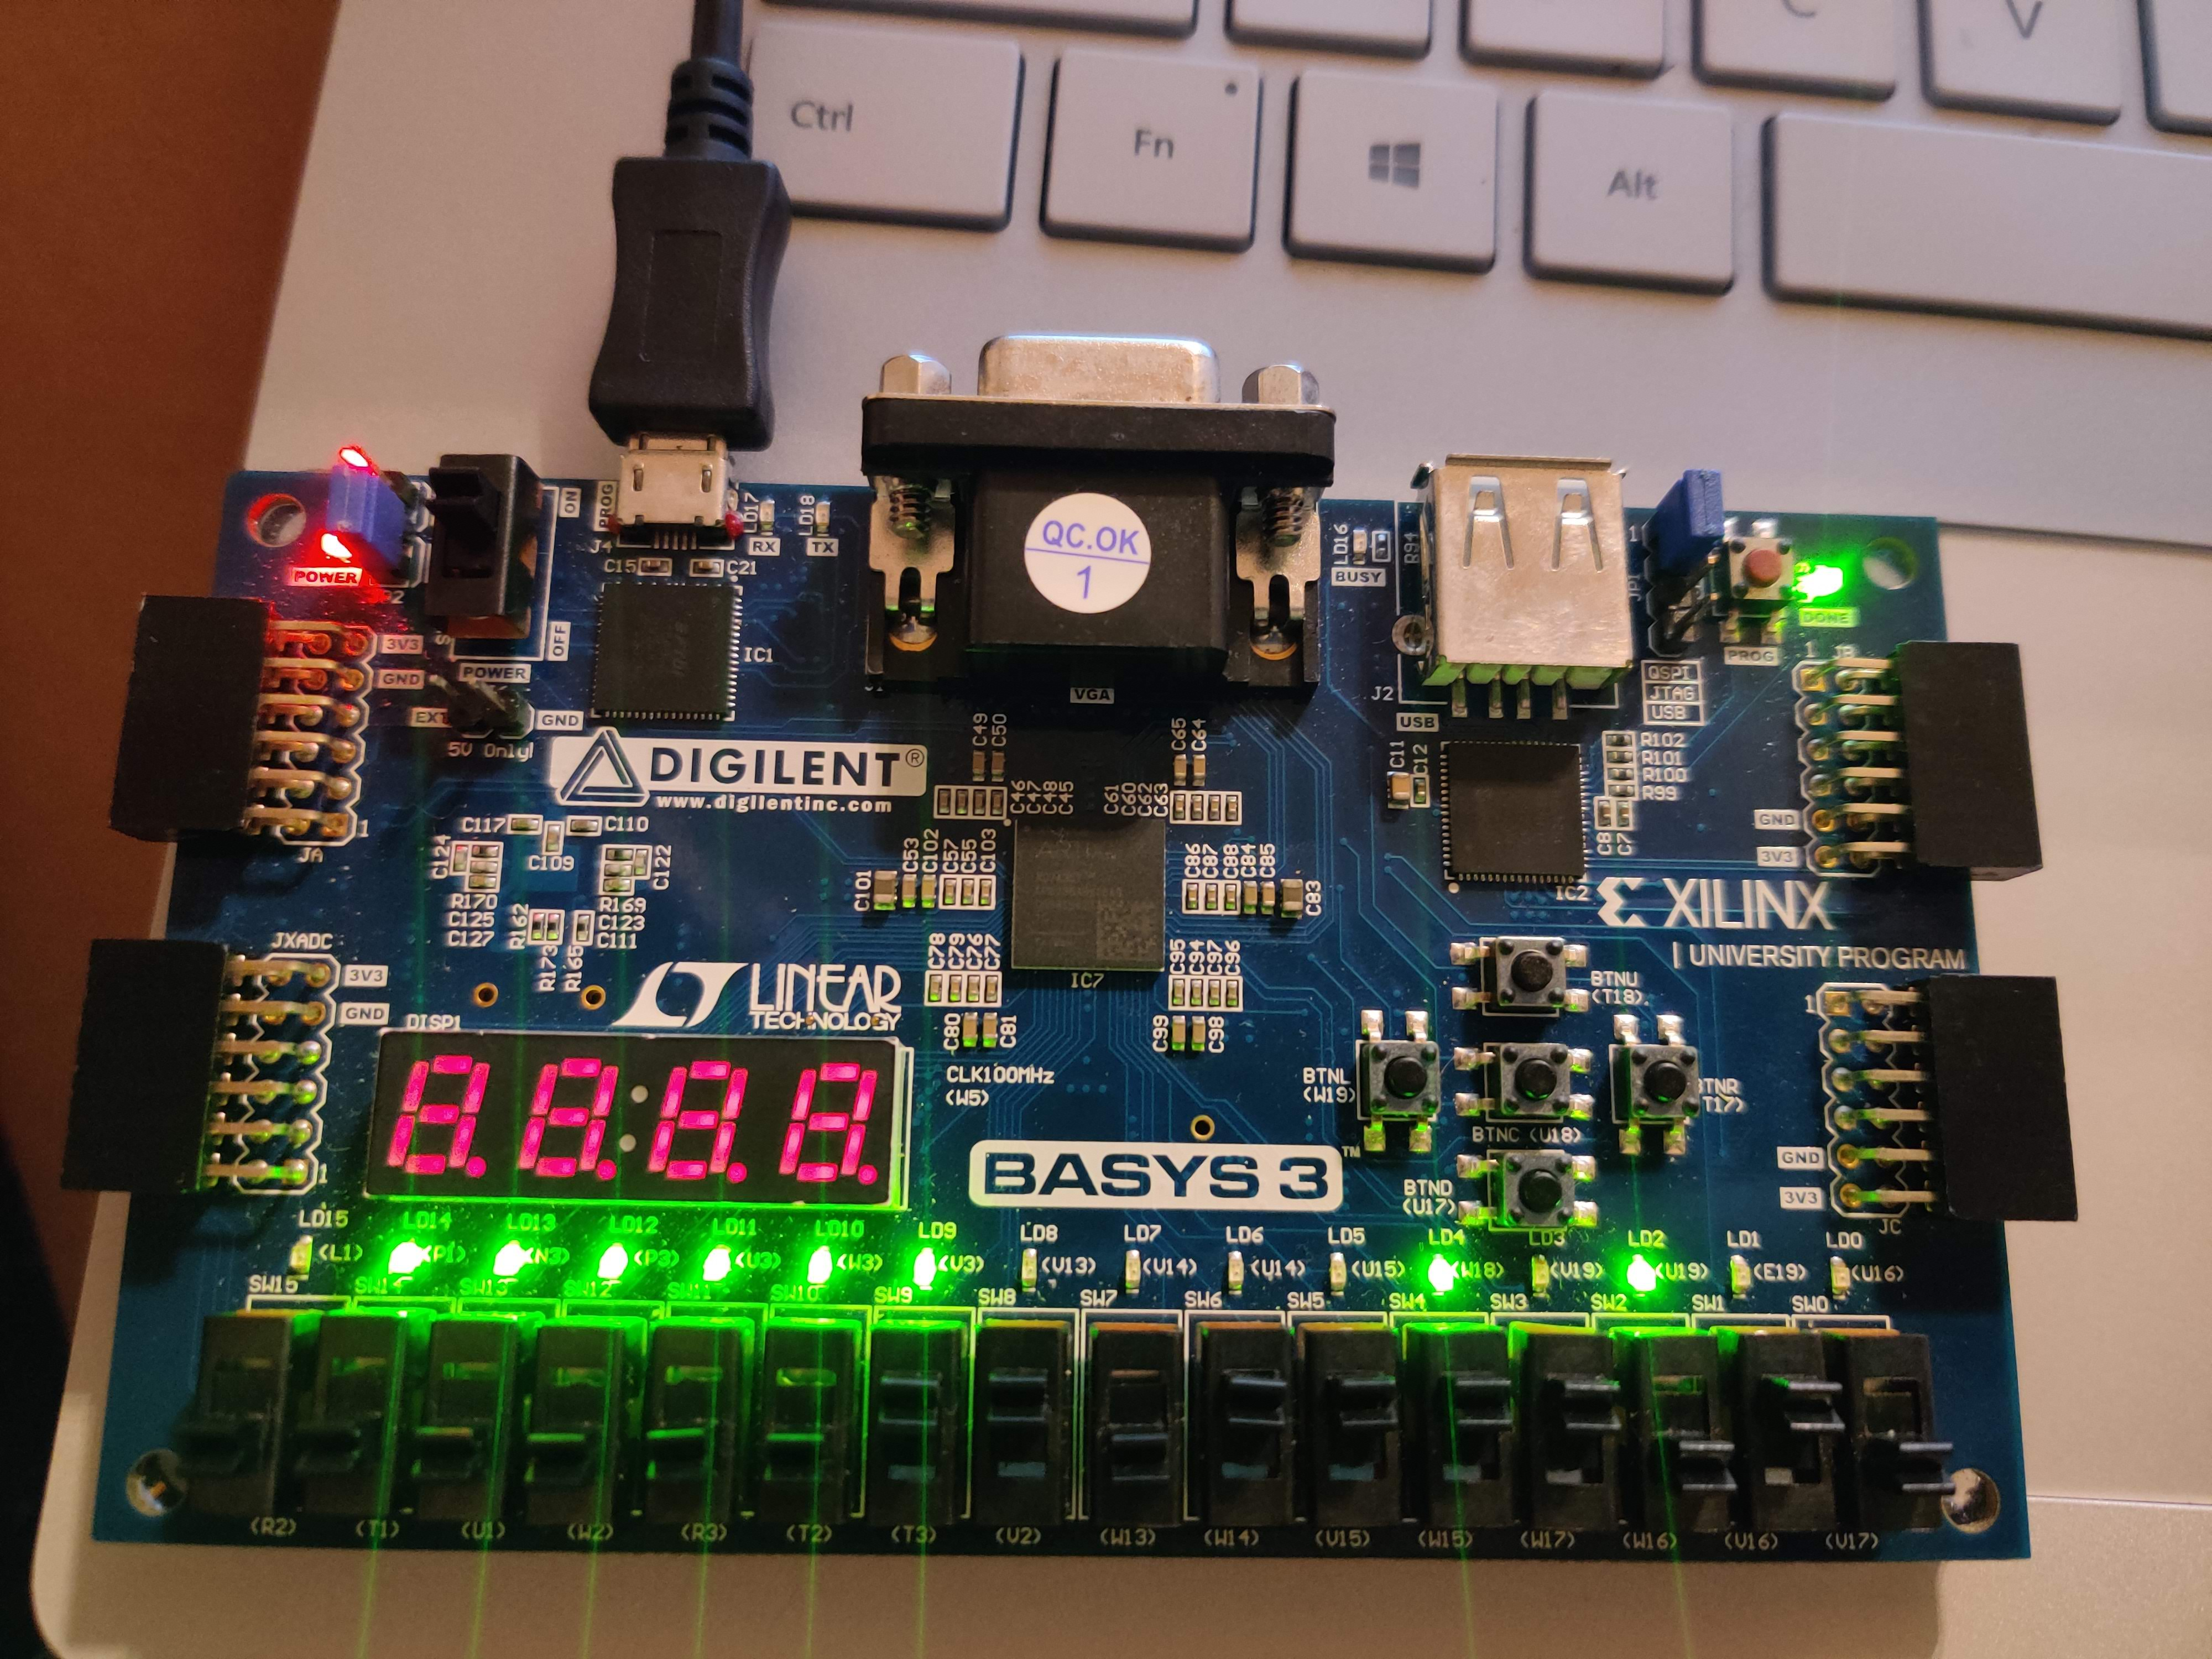
\includegraphics[width=.5\textwidth]{board5}
	\caption{10100 OR 1111010}
	\label{fig:b3_5}			
\end{figure}

\begin{figure}[ht]\centering
	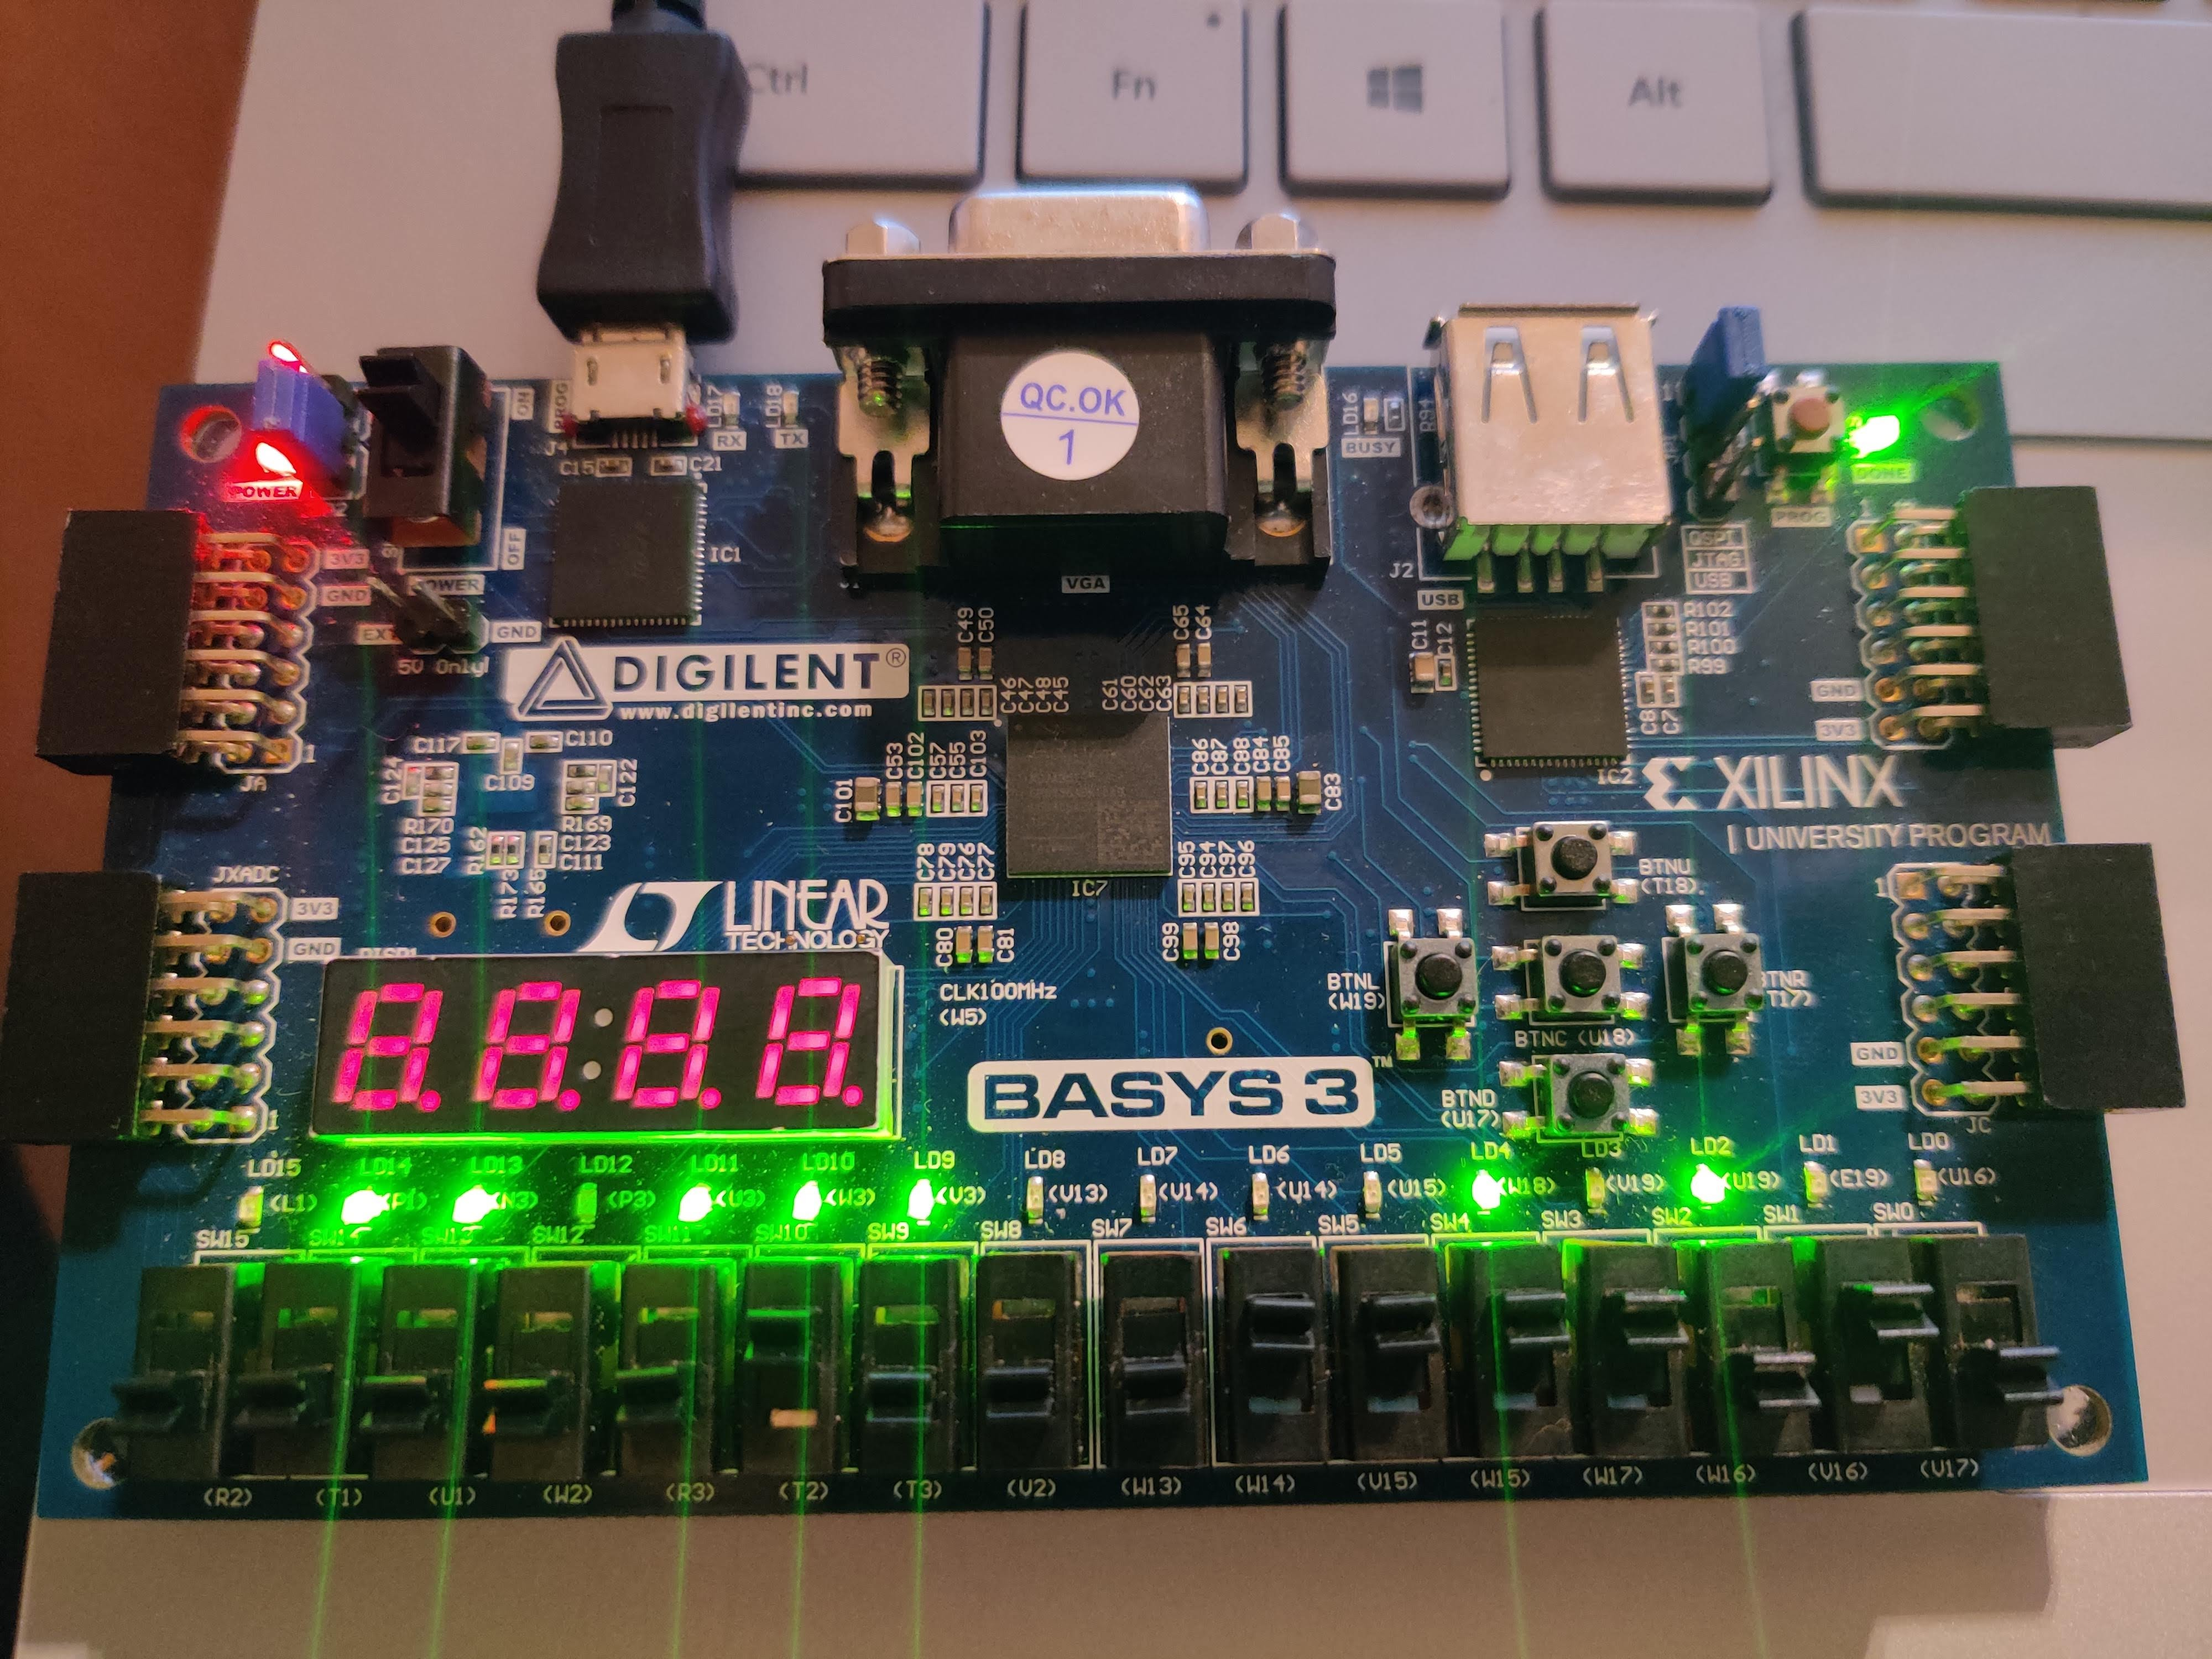
\includegraphics[width=.5\textwidth]{board6}
	\caption{10100 XOR 1111010}
	\label{fig:b3_6}			
\end{figure}

\begin{figure}[ht] \centering	
	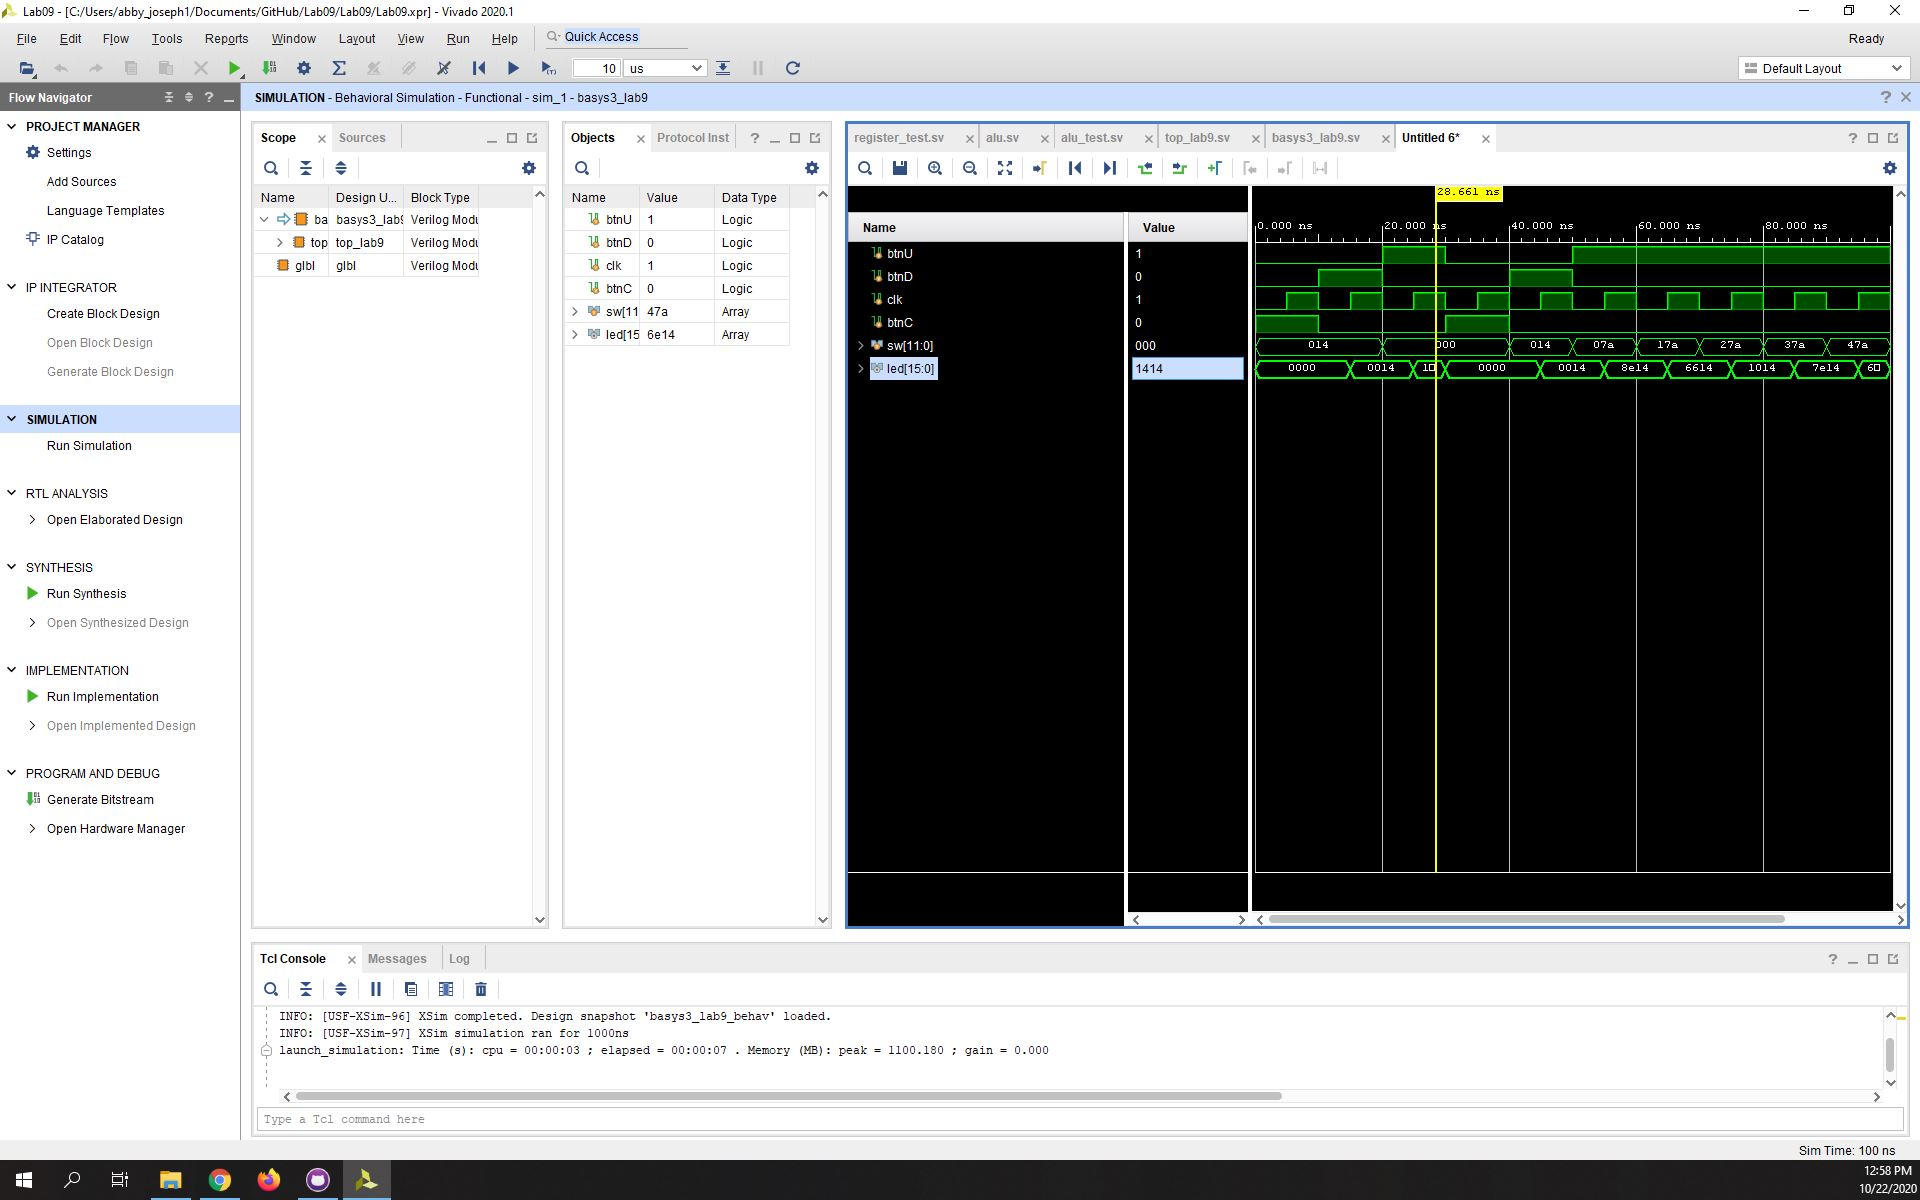
\includegraphics[width=1\textwidth,trim=21cm 19cm 0cm 6cm,clip]{basys3_sim_scrn}
	\caption{Basys3 Simulation}
	\label{fig:img3}
\end{figure}

\end{document}
